\documentclass[border=4pt]{standalone}
\usepackage[T1]{fontenc}
\usepackage{helvet}
\renewcommand{\familydefault}{\sfdefault}
\usepackage{graphicx}
\usepackage{caption}
\usepackage{amsmath}
\captionsetup{font={sf,footnotesize},labelfont={sf,bf,footnotesize},justification=justified,singlelinecheck=false}
\begin{document}
\setcounter{figure}{2}
\begin{minipage}{7.20in}
\centering
\begin{figure}[htbp]
    \centering
    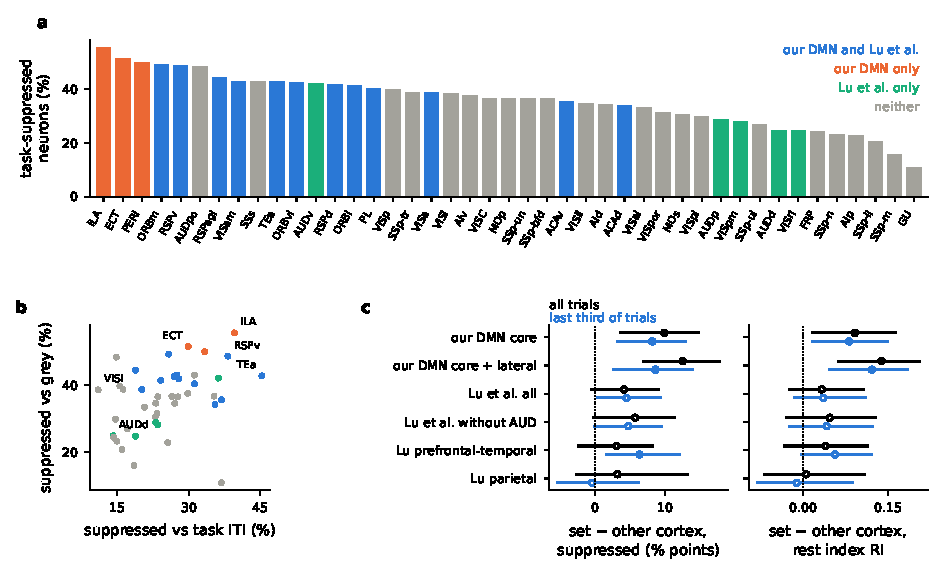
\includegraphics[width=\linewidth]{fig3_restpref_panels.pdf}
    \caption{\textbf{a} Percentage of neurons per cortical region (Beryl) significantly suppressed during the task (movement onset, movement and feedback windows) relative to still 0.3 s chunks of the grey-screen period (Welch test with one chunk per 3 s, p $<$ 0.01; 53,213 neurons, 395 sessions, 130 mice). Colour: membership in our mouse DMN definition (ACA, PL, ILA, ORB, RSP, VISa, VISam + TEa, ECT, PERI) and in the rat DMN of Lu et al. (2012) mapped to mouse regions (ORB, PL, ACA, AUDp/d/v, TEa, VISa, VISrl, RSP, VISam, VISpm; CA1 not shown). \textbf{b} Per region, the same measure referenced to task ITIs (earlier report) against the grey-screen reference; Spearman $\rho$ = 0.44 over 43 regions. \textbf{c} Difference between each region set and all other cortex in the suppressed fraction (left) and in the continuous rest index RI = (rest $-$ task)/(rest + task) (right), against all trials (black) or only the last third of trials, closest in time to the grey screen (blue): 95\% mouse-bootstrap CI; filled markers, region-permutation p $<$ 0.05. Note that 81\% of neurons differ significantly between grey screen and task, so the suppressed fraction is close to the sign of RI.}
    \label{fig:grey_restpref}
\end{figure}
\end{minipage}
\end{document}
